% !TeX spellcheck = en_US
\documentclass[12pt]{article}


\usepackage[english]{babel}
\usepackage[utf8]{inputenc}
\usepackage{graphicx}
\usepackage{amsmath}
\usepackage{mathtools}
\usepackage{hyperref}
\usepackage{biblatex}
\addbibresource{prediction.bib}

\hypersetup{
	colorlinks   = true,    % Colours links instead of ugly boxes
	urlcolor     = blue,    % Colour for external hyperlinks
	linkcolor    = blue,    % Colour of internal links
	citecolor    = red      % Colour of citations
}
\DeclarePairedDelimiter{\ceil}{\lceil}{\rceil}



%opening
\title{Predicting Traffic Patterns in\\ Software Defined Networks}

\author{
	Liva Giovanni - liva.giovanni@spes.uniud.it
	\and
	Hermann Hellwagner - hermann.hellwagner@itec.uni-klu.ac.at
	\and
	Marino Miculan - marino.miculan@uniud.it
}

\date{\today} 

\begin{document}
	
\maketitle

\begin{abstract}
	Just the prediction part
\end{abstract}

\newpage

\section{Introduction}
The predictability of network traffic is the main aim of the thesis. 
Usually, there are two different category of network prediction: short and long period predictions.
The short forecast is used to guess values in terms of seconds or minutes. 
Instead, the long one is adopted to estimate the future workload. 
Therefore, it favors the possibility to produce better planning and decision.
To be able to predict future load of a network, we have to create a model of its behaviors. 
On the changing of a model we have different characteristics such as the correctness of the prediction and its adaptability.


There are two type of models: \textbf{Supervised} and \textbf{Unsupervised}.
The \textit{Supervised} algorithms takes as a input a set of objects and the desired output. 
The set of objects it is called training data.
The learning algorithm analyzes the training data and produces an inferred function that its behavior is checked with the last input. 
The internal structure of the model is changed according to the error between the forecast and the desired result.
Instead, the \textit{Unsupervised} learning tries to find hidden structure in unlabeled data. 
The difference with the \textit{Supervised} learning algorithms is that there is no error or reward signal to evaluate a potential solution.


We focus over the long term prediction and only on supervised classifier.
The decision of which classifier chose has been taken conducting an experiment in a small simulated network. 
We simulate a normal scenario of daily network usage through a network of 4 nodes. 
We repeat the simulation thirty times collecting at each execution statistics of the links utilization in terms of network bandwidth and the load of the switches.
From this information, we have created different dataset changing the features used and the numbers of the last observations.
Then, we have tested the prediction precision and recall of different algorithm at the varying of the distinct datasets. 
\begin{figure}[h!]
	\centering
	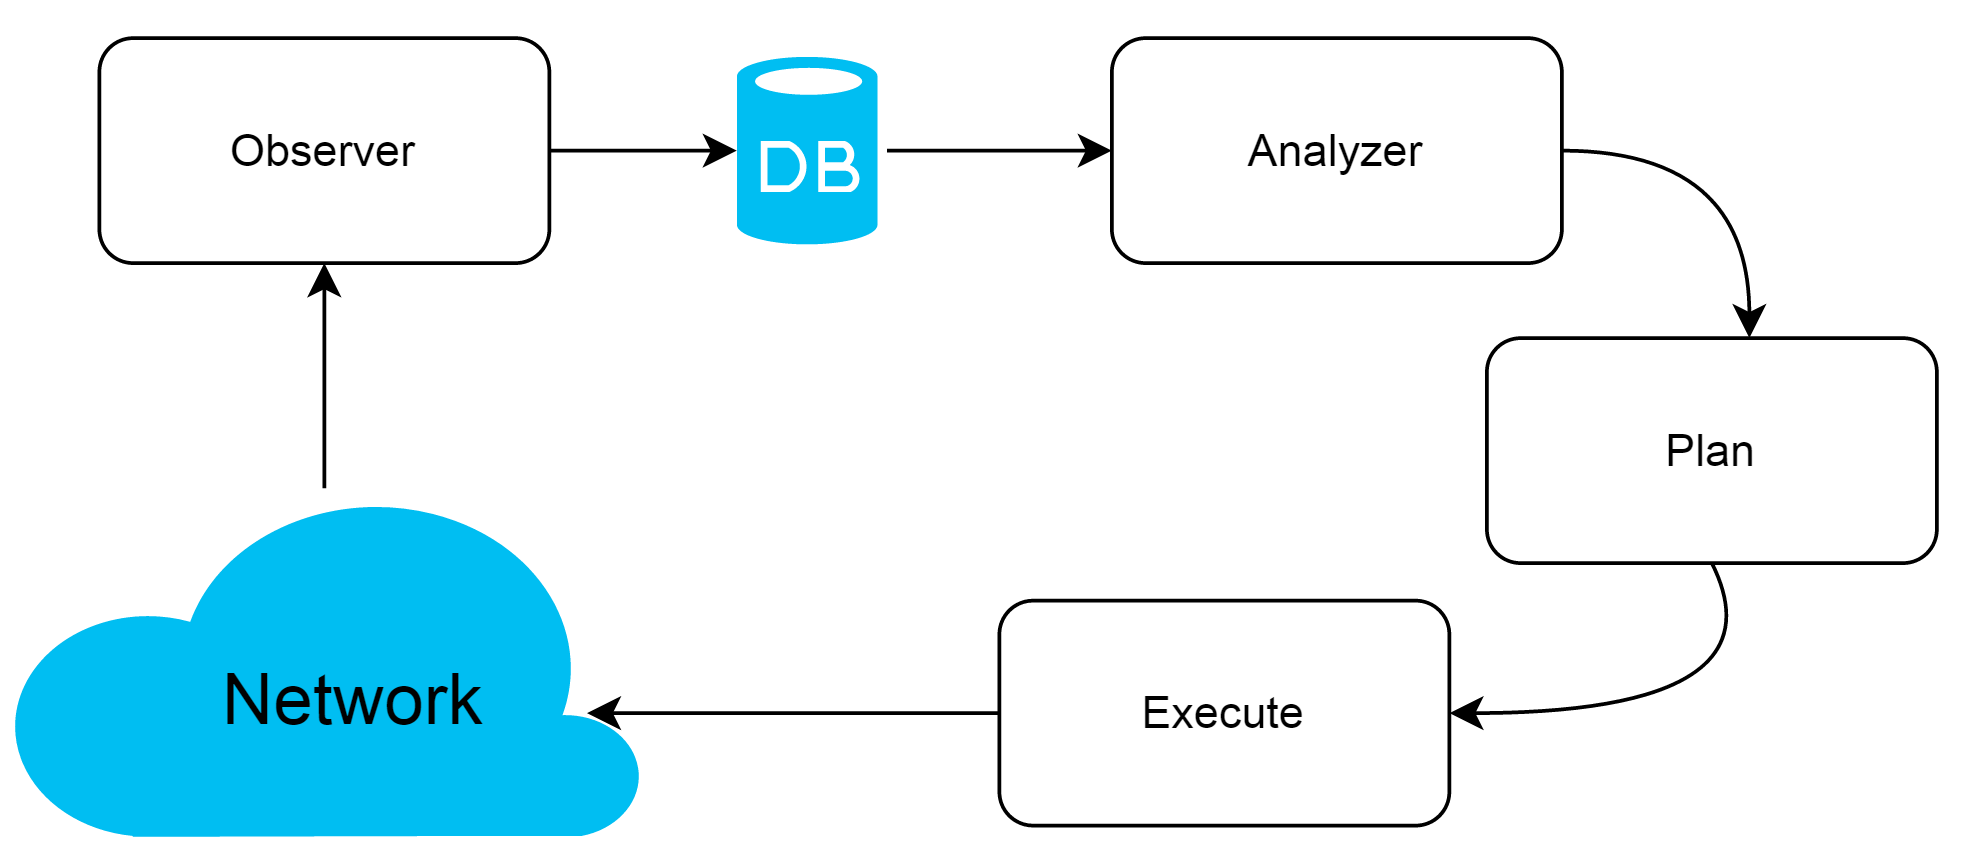
\includegraphics[width=1\textwidth]{img/predictionGraph.png}
	\caption[]
	{The different phases of the prediction}
	\label{fig:predictionConf}
\end{figure}


The implementation of the prediction is designed in four different phases
\begin{itemize}
	\item Observer
	\item Analyzing
	\item Plan
	\item Execute
\end{itemize}
A graphical representation how the four module are interconnected is given in Figure \ref{fig:predictionConf}.\\
The first module, \textbf{Observer}, is implemented as a daemon in the cloud application. 
Every few minute it launches a python script which queries the network controller and then stores the result inside the database.
The information saved regards the network load, switches and flows.


The second one, \textbf{Analyzing}, is done looking through the information inside the database. 
A java application collects the data from the database and converts the knowledge in the Attribute-Relation File Format (ARFF). 
This format is an ASCII text file that describes a list of instances sharing a set of attributes.
The application depends on the $weka$ (Waikato Environment for Knowledge Analysis) package, a well known suite of learning machine algorithms developed by the University of Waikato.
The ARFF files are read by the weka package and used to produce the model that is adopted to make predictions.


The third element, \textbf{Plan}, is demanded to the Administrator.
He or she can write rules to specify what to do when a particular event occurs.
In the cloud application the administrator has the possibility to create the rules that are stored inside the FloodLight controller.


The last phase, \textbf{Execute}, is implemented by the controller. 
It monitors the network and every few minutes it makes predictions using the previously generated model.
When it perceives from a forecast that some rules can be applied, it fires them.


Every module is uncoupled from the others. 
This design decision of modularity gives us the possibility to change or upgrade every module whenever there is the necessity.
This feature is crucial for the prediction phase.
We can test new classifiers or the addiction of new features in a separate and controlled network without affecting the production one. Moreover, we can hot swapping the model using the cloud interface.
We have designed the controller to work with a different model for each switch. 
This decision brings the possibility to predict when a particular node will be overloaded with more precision and recall.\\

 







\section{Prediction over the Network}
\subsection{Configuration}
We have set up a small simulation to decide which classifier algorithm works better for our purpose.
The candidates were the following:
\begin{itemize}
	\item $NaiveBayes$ \cite{naiveBayes}: is a classifier based on the Bayes theorem. It assumes independence between the features of the model. It is in the family of simple probabilistic classifiers.
	\item $SMO$ \cite{smo1,smo2,smo3}: It is an algorithm that employs the support vector machines. The classifier learns by solving an optimization problem.
	\item $BayesNet$ \cite{BayesNet}: It uses the K2 learning algorithm that is in the family of the Naive Bayes. It uses a hill climbing algorithm restricted by an order on the variables of the model.
	\item $MultilayerPerceptron$ \cite{MPL1,MPL2}: It is the most known application of the neural network that uses the back-propagation technique to adjust its internal structure.
	\item $J48$: It is a java implementation of the C4.5 \cite{j48} decision tree algorithm.
	\item $K^*$ ($KStar$) \cite{kstar}: It is an instance-based classifier. It classifies a new instance using the one that is more near to one it has learned in terms of entropy.
	\item $ZeroR$:  This is the dumbest classifier of the list. We have chosen to test it so we can measure other classifiers by how well they do compared to this minimal level of performance. Given a certain data set, ZeroR permits to find out what is the minimum performance we may expect.
\end{itemize}


\begin{figure}[h!]
	\centering
	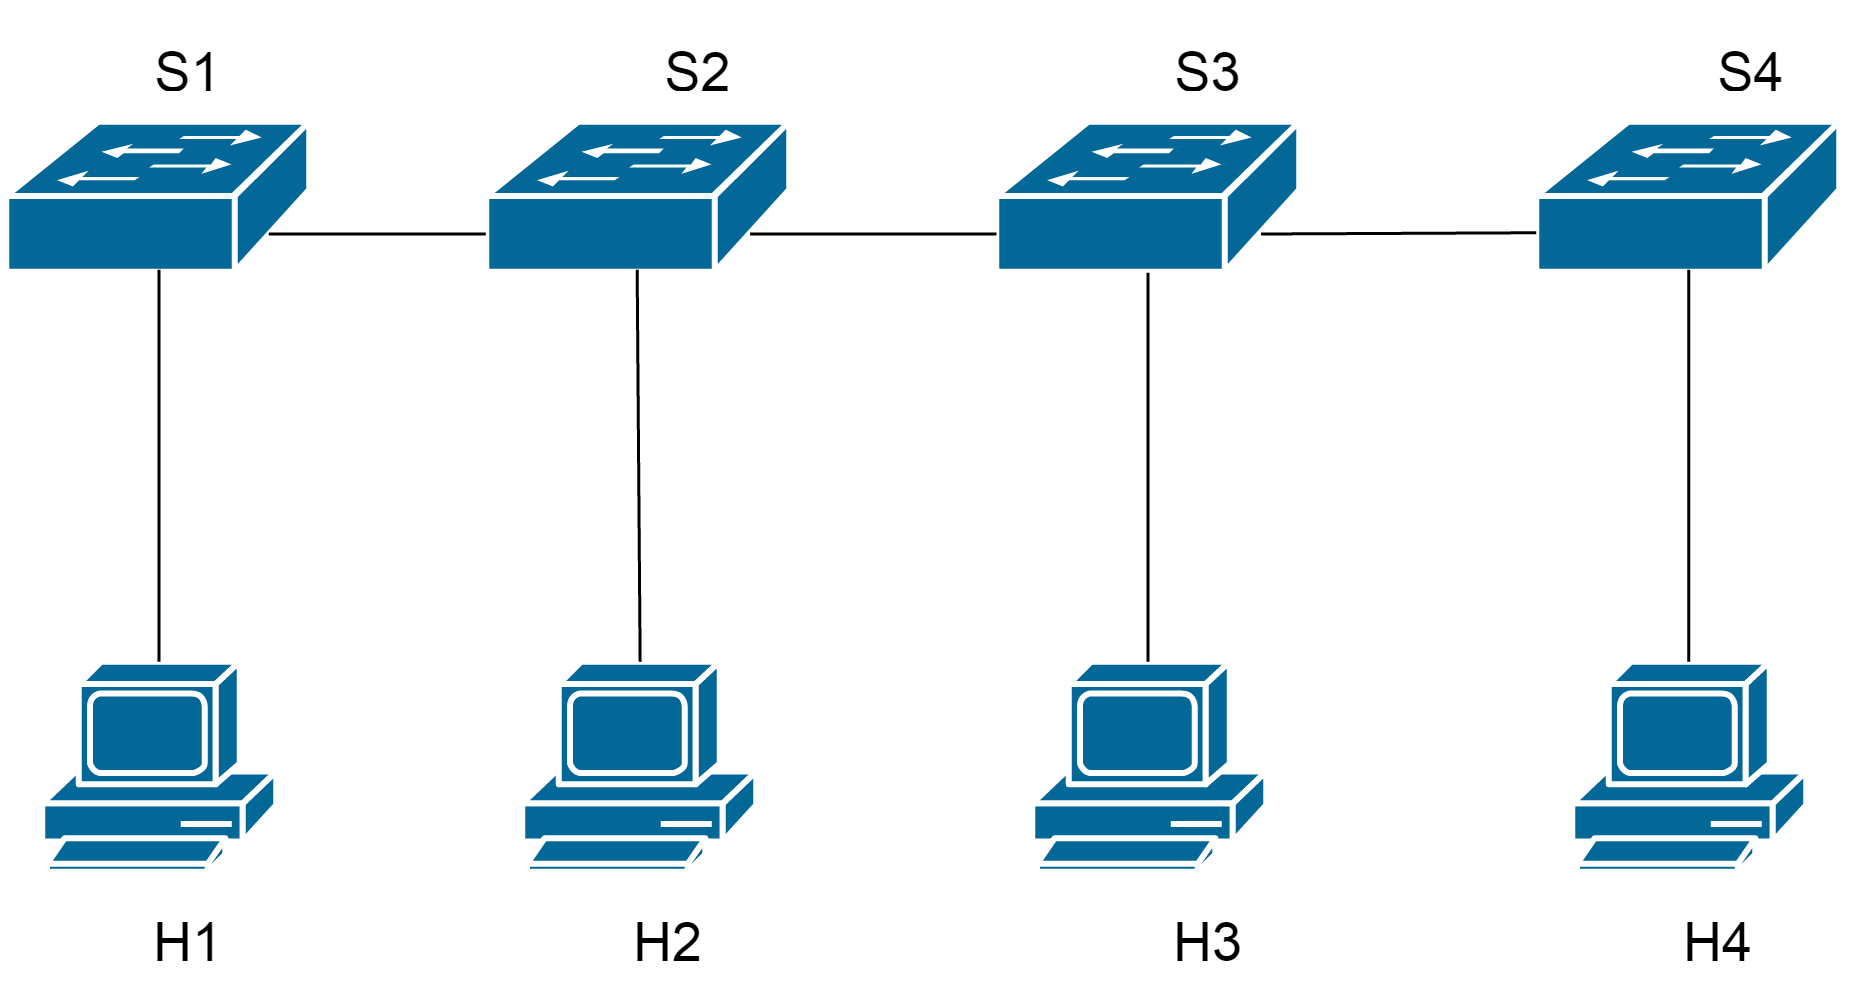
\includegraphics[width=.7\textwidth]{img/networkTopologyScenario.png}
	\caption[]
	{Topology of the network used to test the different classifiers}
	\label{fig:netScenatioTopo}
\end{figure}

\begin{figure}[h!]
	\centering
	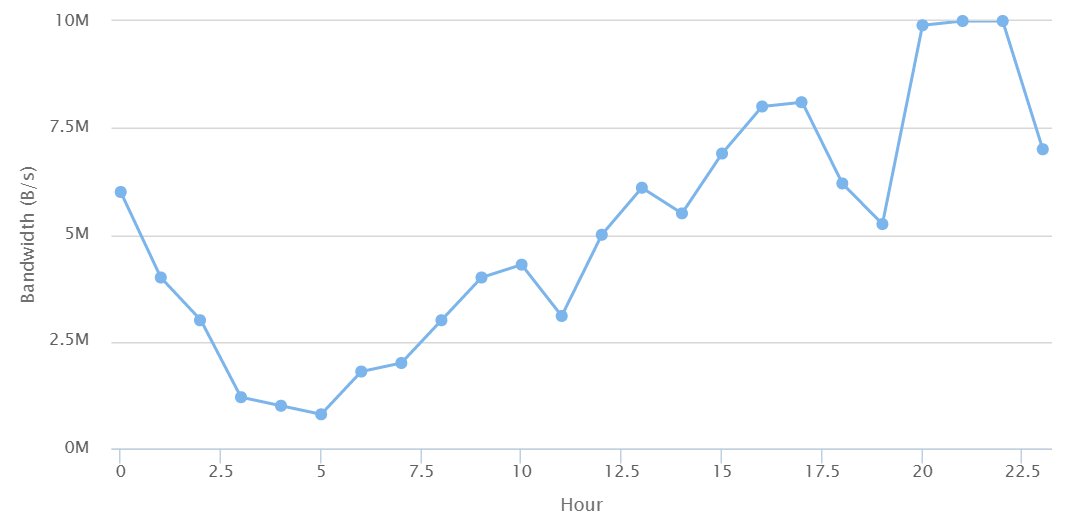
\includegraphics[width=1\textwidth]{img/networkScenario.png}
	\caption[]
	{Graph of the bandwidth simulation of a daily usage of the network}
	\label{fig:netScenarioConf}
\end{figure}


To found the most promising classifier, we have created a network of 4 nodes shows in Figure \ref{fig:netScenatioTopo}.
In this network we have generate traffic from the node $H1$ directed to $H4$ for a day respecting to the scenario predefined. The graph bandwidth generated is shown in Figure \ref{fig:netScenarioConf}.

The creation of the network relies on the virtualization of the hardware components.
Therefore, we have simulated it using Mininet \cite{mininet} with OpenFlow \cite{openflow} switches.
The chosen controller is FloodLight \cite{floodlight}, an open source controller for Software Defined Network.
Regarding the Observer we have created a python script that queries the controller saving the information bla bla bla

%%%%%%%%%%%%%%%%%%%%%%%%%%%%%%%%%%%%%%%%%%%%%%%%%%%%%%%%%%%%%%%%%%%
.\\



Net -> Mininet\\
Observer -> Daemon
Analyzer -> Weka -> Struttura modulare -> Cambiare algo quando si vuole
Plan -> Operator w/ Web Interface config the FloodLight Module
Execute -> FloodLight Module exe the rules
\subsection{DataSet}
%come è stato costruito nel dettaglio
\subsection{Evaluation}
classification learning is appropriate for any problem where deducing a classification is useful and the classification is easy to determine.
%parlare dell'errore come lo calcoliamo noi
\subsection{Result}
Printare i dati in excell, dare qualche valore
\subsection{Discussion}
Avere 50\% di successo -> 10 volte meglio di sparare a caso $1/21 = 4.76\%$

\printbibliography 

	
\end{document}